\chapter{Zufallsvariablen}

Oft sind wir bei der Durchführung von Zufallsexperimenten an gewissen Ereignissen oder Merkmalen 
interessiert. Zum Beispiel an der Anzahl Kopf in drei Münzwürfen.

\begin{definition}
    Eine \textbf{Zufallsvariable} ist eine Abbildung $X : \Omega \rightarrow \mathbb{R}$, wobei $\Omega$
    die Ereignismenge eines Wahrscheinlichkeitsraums ist. Wir definieren die Kurzschreibweise für
    Zufallsvariablen wie folgt:

    $$X \leq 5  := \{\omega \in \Omega | X(\omega) \leq 5\}$$

    Diese Schreibweise steht für das Ereignis, dass die Zufallsvariable $X$ einen Wert kleiner gleich
    5 annimmt.
\end{definition}
\bigskip

Wenn wir nun solch eine Zufallsvariable habe, können wir zwei wichtige Funktionen definieren:

\begin{definition}
    Wir definieren die \textbf{Dichtefunktion} einer Zufallsvariablen $X$ als
    $$f_X : \mathbb{R} \rightarrow [0, 1], x \mapsto \text{Pr}[X = x]$$
    Wir definieren die \textbf{Dichtefunktion} einer Zufallsvariablen $X$ als

    $$F_X : \mathbb{R} \rightarrow [0, 1], x \mapsto \text{Pr}[X \leq x'] = \sum_{x' \in W_x : x \leq x'} \text{Pr}[X = x']$$

    Wobei $W_x = \{x_1, ... , x_n\}$ der Wertebereich der Zufallsvariable ist.
\end{definition}
\pagebreak

\begin{figure}[h]
    \centering
    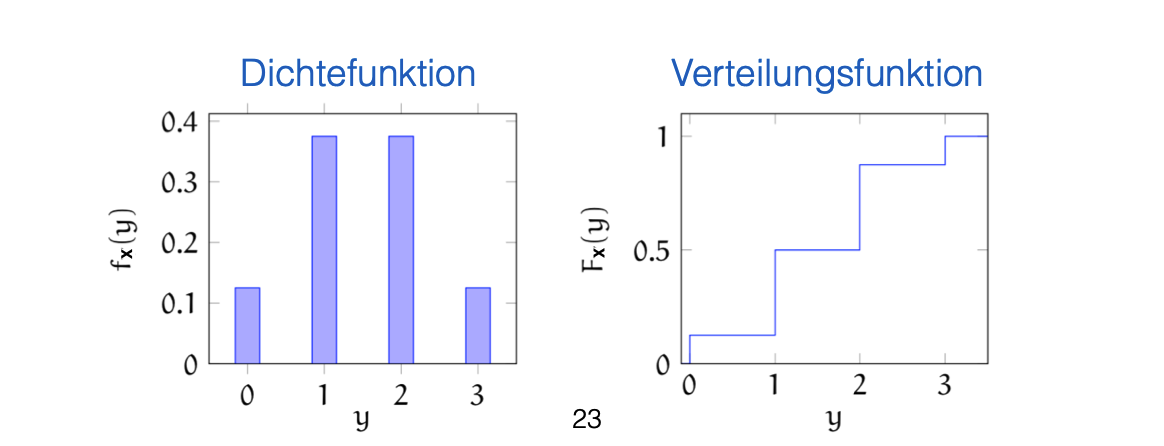
\includegraphics[width=\textwidth]{dichte_verteilungsfunktion.png}
    \caption{Beispiel von Dichte- und Verteilungsfunktion}
\end{figure}
 
\section{Erwartungswert}

Beim Betrachten von Zufallsvariablen ist es interessant zu wissen, welches Ergebnis man “im Mittel” 
erwarten kann. Wir definieren dazu:

\begin{definition}
    Zu einer Zufallsvariablen $X$ definieren wir den \textbf{Erwartungswert} $\mathbb{E}[X]$ durch

    $$\mathbb{E}[X] := \sum_{x \in W_x} x \cdot \text{Pr}[X = x]$$

    oder als alternative Definition

    $$\mathbb{E}[X] := \sum_{\omega \in \Omega} X(\omega) \cdot \text{Pr}[\omega]$$

    Wobei zu erwähnen ist, dass wir in der Vorlesung nur Zufallsvariablen betrachten, wo auch wirklich
    ein Erwartungswert existiert.
\end{definition}
\bigskip

Für ganzzahlige, positive Wertebereiche, können wir den Erwartungswert wie folgt berechen:

\begin{satz}[Satz]
    Sei $X$ eine Zufallsvariable mit $W_X \subseteq \mathbb{N}_0$, dann gilt

    $$\mathbb{E}[X] = \sum_{i=1}^\infty \text{Pr}[X \geq i]$$
\end{satz}
\bigskip

Eine wichtige Eigenschafft des Erwartungswertes ist seine Linearität.

\begin{satz}[Linearität des Erwartungswertes]
    Für Zufallsvariablen $X_1, ... , X_n$ und $X = \alpha_1 \cdot X_1 + ... + \alpha_n \cdot X_n + \beta$
    mit $\alpha_1, ..., \alpha_n, \beta \in \mathbb{R}$ gilt

    $$\mathbb{E}[X] = \alpha_1 \cdot \mathbb{E}[X_1] + ... + \alpha_n \cdot \mathbb{E}[X_n] + \beta$$
\end{satz}
\bigskip

An dieser Stelle lohnt es sich auch den Begriff der Indikatorvariable einzuführen.

\begin{definition}
    Für ein Ereignis $A \subseteq \Omega$ ist die zugehörige \textbf{Indikatorvariable} $X_A$ definiert
    durch:

    $$X_A(\omega) := \begin{cases}
        1, \text{ falls }(\omega) \in A\\
        0, \text{ sonst }
    \end{cases}$$

    Für den Erwartungswert von $X_A$ gilt: $\mathbb{E}[X_A] = \text{Pr}[A]$.
\end{definition}

